\section{\textbf{Introduction}}

\subsection{\textbf{Problem Background}}
Artificial light at night (ALAN) has added great value to our lives, while the excessive or poor use of it has contributed to light pollution. Though some studies consider the reflection of glass curtain wall as part of light pollution\textsuperscript{\cite{ref1}}, we concentrate on the light pollution caused by excessive or poor use of artificial light under the given topic, ALAN in particular. ALAN data from satellites provide us with a direct insight on light pollution\textsuperscript{\cite{ref2}}. It is easy to find that the higher light pollution (represented by brighter color) centred on area with higher levels of social-economic and urbanization. \par 
Light pollution has environmental impacts and affects our health and safety proven by previous researches\textsuperscript{\cite{ref3},\cite{ref4}}, leading to the demand for a comprehensive metrics to assess the impact of light pollution on environment and human health. \par 
\begin{figure}[ht]
    \centering
    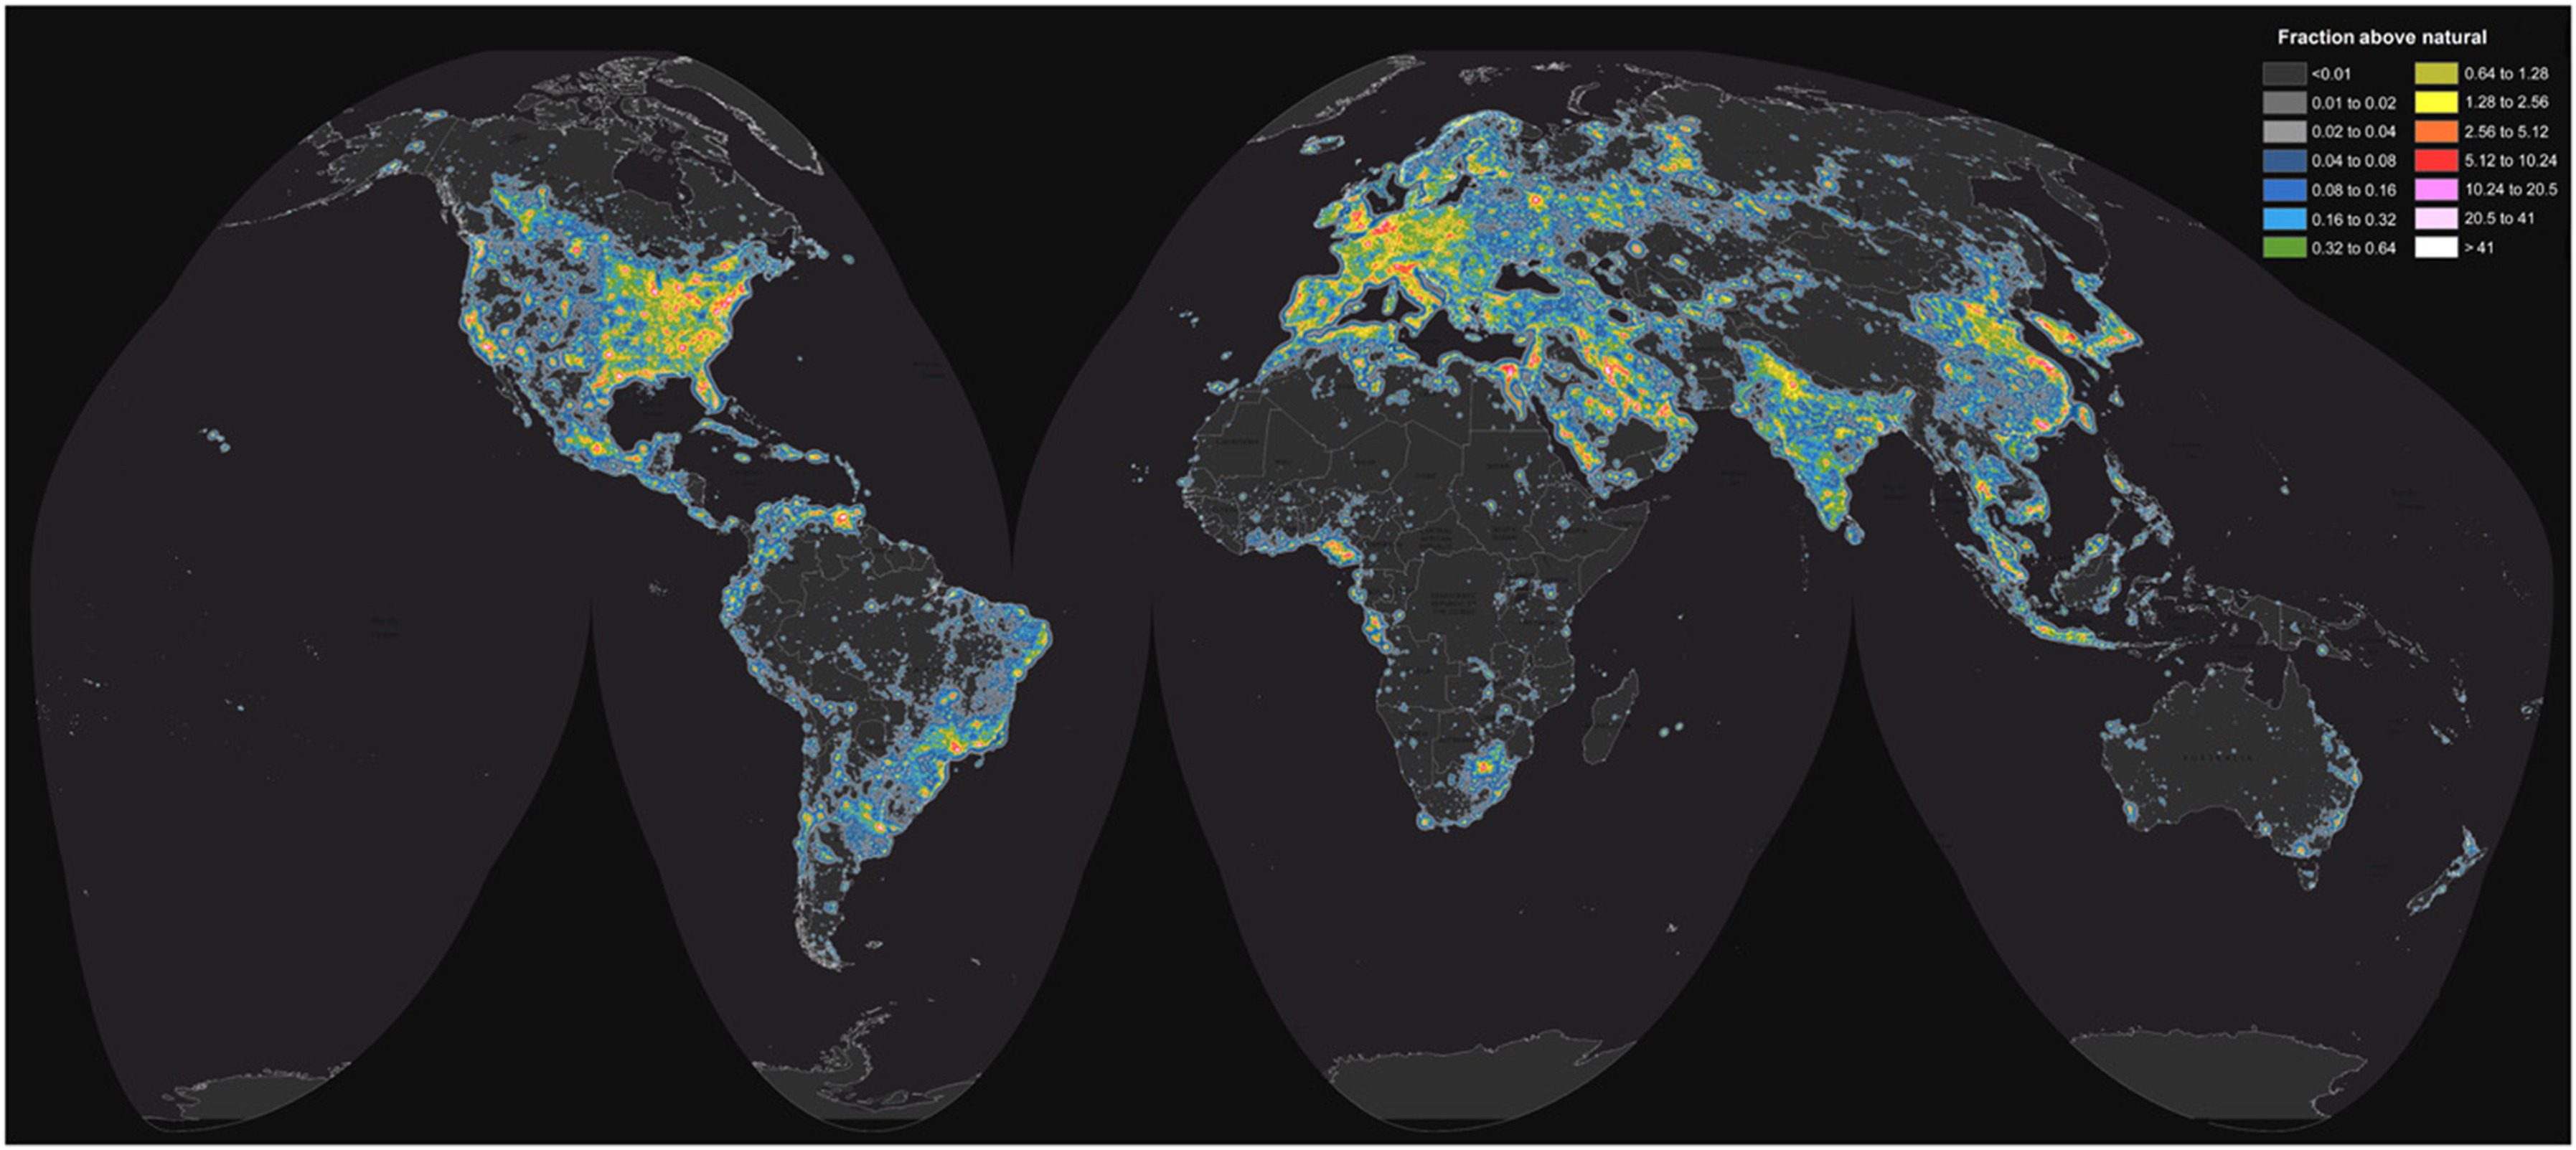
\includegraphics[width=\textwidth]{../pictures/1 Introduction/1 satellite data.jpg}
    \caption{World atlas of artificial sky brightness created using satellite data by Falchi et al.}
\end{figure}

\subsection{\textbf{Our work}}
We develop a comprehensive metrics to estimate the impacts of light pollution concerning environment and human health with Analytic Hierarchy Process (AHP).\par 
